\\
\titre{Problème producteur / consommateur : } On a $n$ processus ou threads qui produisent des données. Ces données sont traitées par $m$ autres processus ou threads. (souvent $n > 1$ et $m = 1$. Exemple : le spool d'impression). \\
Solution naïve :
\begin{itemize}
	\item Données : 
	\begin{itemize}
		\item un tableau Tab de taille $N$. (dans lequel les producteurs écrivent et les consommateurs lisent)
		\item un entier lib représentant l'indice de la première case libre pour écrire
		\item un entier occ représentant l'indice de la première case occupée pour lire
		\item un entier nbocc indiquant le nombre de cases occupées.
		\item un entier nblib indiquant le nombre de cases libres.
	\end{itemize}
	\item Initialisation :
	\begin{itemize}
		\item lib et occ valent 0, nb\_lib = N et nb\_occ = 0.
	\end{itemize}
	\item Producteur : \\
\\ 
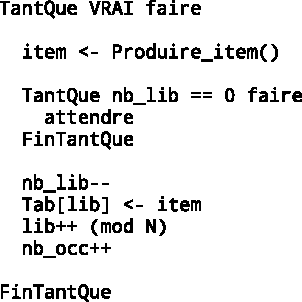
\includegraphics{fig12.pdf}
	\item Consommateur : \\
\\ 
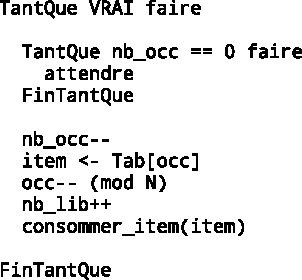
\includegraphics{fig13.pdf}
\end{itemize}

\titre{Sémaphore :} (Dijkstra 1965) Un entier muni de deux fonctions \titre{POST} et \titre{WAIT} et une file d'attente. La file d'attente contient des processus ou threads bloqués sur le sémaphore. \\
\begin{itemize}
	\item POST : \\
\\ 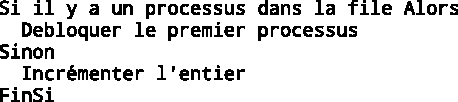
\includegraphics{fig14.pdf}
	\item WAIT : \\
\\ 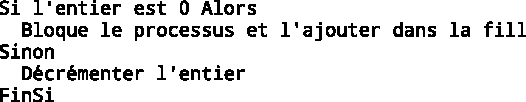
\includegraphics{fig15.pdf}
	\item Contrainte : Les fonctions POST et WAIT doivent être implémentées de manière à ne jamais être interrompues. On parle d'une solution matérielle ET logicielle.
	\item Lorsqu'un processus est bloqué il ne consomme aucun temps CPU
	\item Lorsque des processus sont bloqués sur le sémaphore, son entier vaut forcément 0 (la réciproque est fausse)
\end{itemize}

\titre{Solution à l'exclusion mutuelle :} \\
\\	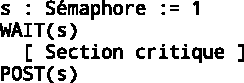
\includegraphics{fig16.pdf} \\
\titre{Solution du producteur / consommateur :}
\begin{itemize}
	\item Données : 
	\begin{itemize}
		\item un tableau Tab de taille $N$. (dans lequel les producteurs écrivent et les consommateurs lisent)
		\item un entier lib représentant l'indice de la première case libre pour écrire
		\item un entier occ représentant l'indice de la première case occupée pour lire
		\item un sémaphore nbocc qui compte les cases occupées
		\item un sémaphore nblib qui compte les cases libres
		\item un sémaphore excl pour gérer l'exclusion mutuelle
	\end{itemize}
	\item Producteur : \\
\\ 
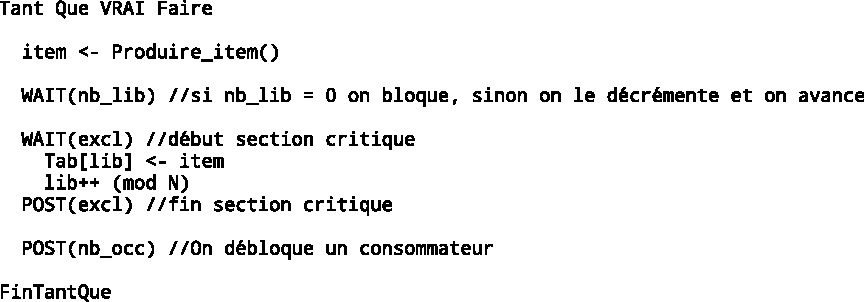
\includegraphics{fig17.pdf}
	\item Consommateur : \\
\\ 
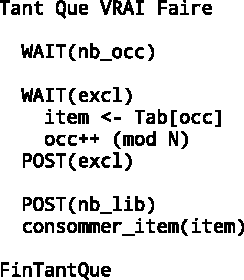
\includegraphics{fig18.pdf}
\end{itemize}

\titre{Mutex :} Sémaphore binaire servant uniquement à assurer l'exclusion mutuelle. L'entier est remplacé par deux états possibles : verrouillé ou déverrouillé. Les 2 fonctions s'appellent alors LOCK et UNLOCK \\

\titre{Sémaphore nommé / non nommé :} Un sémaphore nommé apparait dans le système de fichier (plusieurs processus qui ne se connaissent pas peuvent l'utiliser) (c'est un fichier virtuel, les droits d'accès s'appliquent).  Un sémaphore non nommé est simplement une variable de notre processus (partagée entre nos threads uniquement).

